%%%%%%%%%%%%%%%%%%%%%%%%%%%%%%%%%%%%%%%%%%%%%%%%%%%%%%%%%%%%
%%% LIVECOMS ARTICLE TEMPLATE FOR BEST PRACTICES GUIDE
%%% ADAPTED FROM ELIFE ARTICLE TEMPLATE (8/10/2017)
%%%%%%%%%%%%%%%%%%%%%%%%%%%%%%%%%%%%%%%%%%%%%%%%%%%%%%%%%%%%
%%% PREAMBLE
\documentclass[9pt,tutorial]{livecoms}
% Use the 'onehalfspacing' option for 1.5 line spacing
% Use the 'doublespacing' option for 2.0 line spacing
% Use the 'lineno' option for adding line numbers.
% Use the "ASAPversion' option following article acceptance to add the DOI and relevant dates to the document footer.
% Use the 'pubversion' option for adding the citation and publication information to the document footer, when the LiveCoMS issue is finalized.
% The 'bestpractices' option for indicates that this is a best practices guide.
% Omit the bestpractices option to remove the marking as a LiveCoMS paper.
% Please note that these options may affect formatting.

\usepackage{lipsum} % Required to insert dummy text
\usepackage[version=4]{mhchem}
\usepackage{siunitx}
\DeclareSIUnit\Molar{M}
\usepackage[italic]{mathastext}
\graphicspath{{figures/}}

%%%%%%%%%% USER INPUT PACKAGES & FUNCTIONS
\usepackage{listings}
\lstset{
	basicstyle=\ttfamily,
	commentstyle={},
	breakatwhitespace=true,
	breaklines=true,
	language=bash
}
\usepackage{pythonhighlight}

%%%%%%%%%%%%%%%%%%%%%%%%%%%%%%%%%%%%%%%%%%%%%%%%%%%%%%%%%%%%
%%% IMPORTANT USER CONFIGURATION
%%%%%%%%%%%%%%%%%%%%%%%%%%%%%%%%%%%%%%%%%%%%%%%%%%%%%%%%%%%%

\newcommand{\versionnumber}{1.0}  % you should update the minor version number in preprints and major version number of submissions.
\newcommand{\githubrepository}{\url{https://github.com/michellab/BioSimSpaceTutorials}}  %this should be the main github repository for this article

%%%%%%%%%%%%%%%%%%%%%%%%%%%%%%%%%%%%%%%%%%%%%%%%%%%%%%%%%%%%
%%% ARTICLE SETUP
%%%%%%%%%%%%%%%%%%%%%%%%%%%%%%%%%%%%%%%%%%%%%%%%%%%%%%%%%%%%
\title{This is the title [Article v\versionnumber]}

\author[1*]{Firstname Middlename Surname}
\author[1,2\authfn{1}\authfn{3}]{Firstname Middlename Familyname}
\author[2\authfn{1}\authfn{4}]{Firstname Initials Surname}
\author[2*]{Firstname Surname}
\affil[1]{Institution 1}
\affil[2]{Institution 2}

\corr{email1@example.com}{FMS}  % Correspondence emails.  FMS and FS are the appropriate authors initials.
\corr{email2@example.com}{FS}

\orcid{Author 1 name}{AAAA-BBBB-CCCC-DDDD}
\orcid{Author 2 name}{EEEE-FFFF-GGGG-HHHH}

\contrib[\authfn{1}]{These authors contributed equally to this work}
\contrib[\authfn{2}]{These authors also contributed equally to this work}

\presentadd[\authfn{3}]{Department, Institute, Country}
\presentadd[\authfn{4}]{Department, Institute, Country}

\blurb{This LiveCoMS document is maintained online on GitHub at \githubrepository; to provide feedback, suggestions, or help improve it, please visit the GitHub repository and participate via the issue tracker.}

%%%%%%%%%%%%%%%%%%%%%%%%%%%%%%%%%%%%%%%%%%%%%%%%%%%%%%%%%%%%
%%% PUBLICATION INFORMATION
%%% Fill out these parameters when available
%%% These are used when the "pubversion" option is invoked
%%%%%%%%%%%%%%%%%%%%%%%%%%%%%%%%%%%%%%%%%%%%%%%%%%%%%%%%%%%%
\pubDOI{10.XXXX/YYYYYYY}
\pubvolume{<volume>}
\pubissue{<issue>}
\pubyear{<year>}
\articlenum{<number>}
\datereceived{Day Month Year}
\dateaccepted{Day Month Year}

%%%%%%%%%%%%%%%%%%%%%%%%%%%%%%%%%%%%%%%%%%%%%%%%%%%%%%%%%%%%
%%% ARTICLE START
%%%%%%%%%%%%%%%%%%%%%%%%%%%%%%%%%%%%%%%%%%%%%%%%%%%%%%%%%%%%

\begin{document}

\begin{frontmatter}
\maketitle

\begin{abstract}
This particular document provides a skeleton illustrating key sections for a Tutorial document.
Please see the sample \texttt{sample-document.tex} in \url{github.com/livecomsjournal/article_templates/templates} for additional information on and examples of using the LiveCoMS LaTeX class.
Here we also assume familiarity with LaTeX and knowledge of how to include figures, tables, etc.; if you want examples, see the sample just referenced.

In your work, in this particular slot, please provide an abstract of no more than 250 words.
Your abstract should explain the main contributions of your article, and should not contain any material that is not included in the main text.
Please note that your abstract, plus the authorship material following it, must not extend beyond the title page or modifications to the LaTeX class will likely be needed.
\end{abstract}

\end{frontmatter}




\section{Introduction}

Here you would explain what problem you are tackling and briefly motivate your work.

In this particular template, we have removed most of the usage examples which occur in \texttt{sample-document.tex} to provide a minimal template you can modify; however, we retain a couple of examples illustrating more unusual features of our templates/article class, such as the checklists, and information on algorithms and pseudocode.

Keep in mind, as you prepare your manuscript, that you should plan for a representative image  which will be used to highlight your article on the journal website and publications. Usually, this would be one of your figures, but it must also be uploaded separately upon article submission. We give specific guidelines for this image on the journal website in the section on article submission (see \url{https://livecomsjournal.github.io/authors/policies/index.html#article-submission}).

Additionally, for well-formatted manuscripts, we recommend that you let LaTeX handle figure/table placement for you as much as possible, so please avoid specifying strenuous float instructions like `[h!]` and `[H]` as much as possible.

\subsection{Scope}

Tutorials should endeavor to cover the specific task at hand, and also highlight how the steps might need to be modified (or additional care might need to be taken at particular points) to handle more general cases.

The scope of the tutorial, as well as the expected proficiencies / outcomes for researchers who complete the tutorial, should be clearly defined.
This will often happen in a specific section or subsection in the article itself.

\section{Prerequisites}

Here you would identify prerequisites/background knowledge that are assumed by your work, as well as any software/license requirements.

\subsection{Background knowledge}
Tutorials should clearly define what concepts or abilities researchers will need to complete the tutorial (e.g., some proficiency in Python; experience with Jupyter notebooks; knowledge of classical MD; etc).

\subsection{Software/system requirements}
Tutorials should clearly define what system and/or software requirements the researcher will need to complete the tutorial (e.g., VMD version 1.9 or newer, AMBER, etc.). Tutorials requiring specific software packages must provide instructions and files for the referenced version of the software.

\section{Content and links}

A tutorial will normally draw on additional files and materials; clearly indicate where and how these are available, with links, and how they are being archived for the long-term and maintained so they stay current.
You will likely want to reference your GitHub repository as a central point to access all of this information, and then the GitHub repository may link out to other content as needed.

\subsection{Introduction}
\subsection{Funnel Meta-Dynamics}
\subsection{Steered Molecular Dynamics \& Markov State Modeling}
\subsection{Free Energy Perturbation}
%%%%%%%%%%%%%%%%%%%%%%%%%%%%%%%%%%%%%%%%%%%%%%%%%%%%%%%%%%%%%%%%%%%%%%%%%%%%%%%%%%%%%%%%%%%
%%%%%%%%%%%%%%%%%%%%%%%%%%%%%%%%%%%%%%%%%%%%%%%%%%%%%%%%%%%%%%%%%%%%%%%%%%%%%%%%%%%%%%%%%%%
%%%%%%%%%%%%%%%%%%%%%%%%%%%%%%%%%%%%%%%%%%%%%%%%%%%%%%%%%%%%%%%%%%%%%%%%%%%%%%%%%%%%%%%%%%%
%%%%%%%%%%%%%%%%%%%%%%%%%%%%%%%%%%%%%%%%%%%%%%%%%%%%%%%%%%%%%%%%%%%%%%%%%%%%%%%%%%%%%%%%%%%
%%%%%%%%%%%%%%%%%%%%%%%%%%%%%%%%%%%%%%%%%%%%%%%%%%%%%%%%%%%%%%%%%%%%%%%%%%%%%%%%%%%%%%%%%%%
%%%%%%%%%%%%%%%%%%%%%%%%%%.  WRITE YOUR CHAPTER CONTENTS BELOW.  %%%%%%%%%%%%%%%%%%%%%%%%%%
%%%%%%%%%%%%%%%%%%%%%%%%%%%%%%%%%%%%%%%%%%%%%%%%%%%%%%%%%%%%%%%%%%%%%%%%%%%%%%%%%%%%%%%%%%%
%%%%%%%%%%%%%%%%%%%%%%%%%%%%%%%%%%%%%%%%%%%%%%%%%%%%%%%%%%%%%%%%%%%%%%%%%%%%%%%%%%%%%%%%%%%
%%%%%%%%%%%%%%%%%%%%%%%%%%%%%%%%%%%%%%%%%%%%%%%%%%%%%%%%%%%%%%%%%%%%%%%%%%%%%%%%%%%%%%%%%%%

\subsubsection{Introduction}


Computational chemists can support structure-activity relationship
studies in medicinal chemistry by making computer models that can
predict binding affinity of ligands to proteins. One of the most popular
techniques for this is Free Energy Perturbation (FEP), which relies on
simulation alchemical transformations of ligands in a congeneric series,
simulating them both in a protein target and in just a waterbox.
Relative free energies of binding ($\Delta\Delta$G in kcal/mol) can then be computed
by simply subtracting the $\Delta$G (in protein) and the $\Delta$G (in water). Some
introductory reading is recommended. \cite{mey2020best, cournia_allen_sherman_2017, kuhn_firth-clark_tosco_mey_mackey_michel_2020}

This tutorial will outline the steps needed to:

\begin{itemize}
\item
  Select a series of transformations to simulate using LOMAP
\item
  Use BioSimSpace to set up files needed for a standard FEP run in both
  SOMD and GROMACS
\item
  Run FEP using BioSimSpace on a computing cluster
\item
  Analyse FEP simulation results
\item
  Compile all FEP results locally and perform data analyses
\end{itemize}

For this tutorial we will be using TYK2, a common benchmarking set in
the FEP field, first used by Schrödinger in their
\href{https://pubs.acs.org/doi/abs/10.1021/ja512751q}{2015 FEP+ paper}.

\begin{figure}[htp]
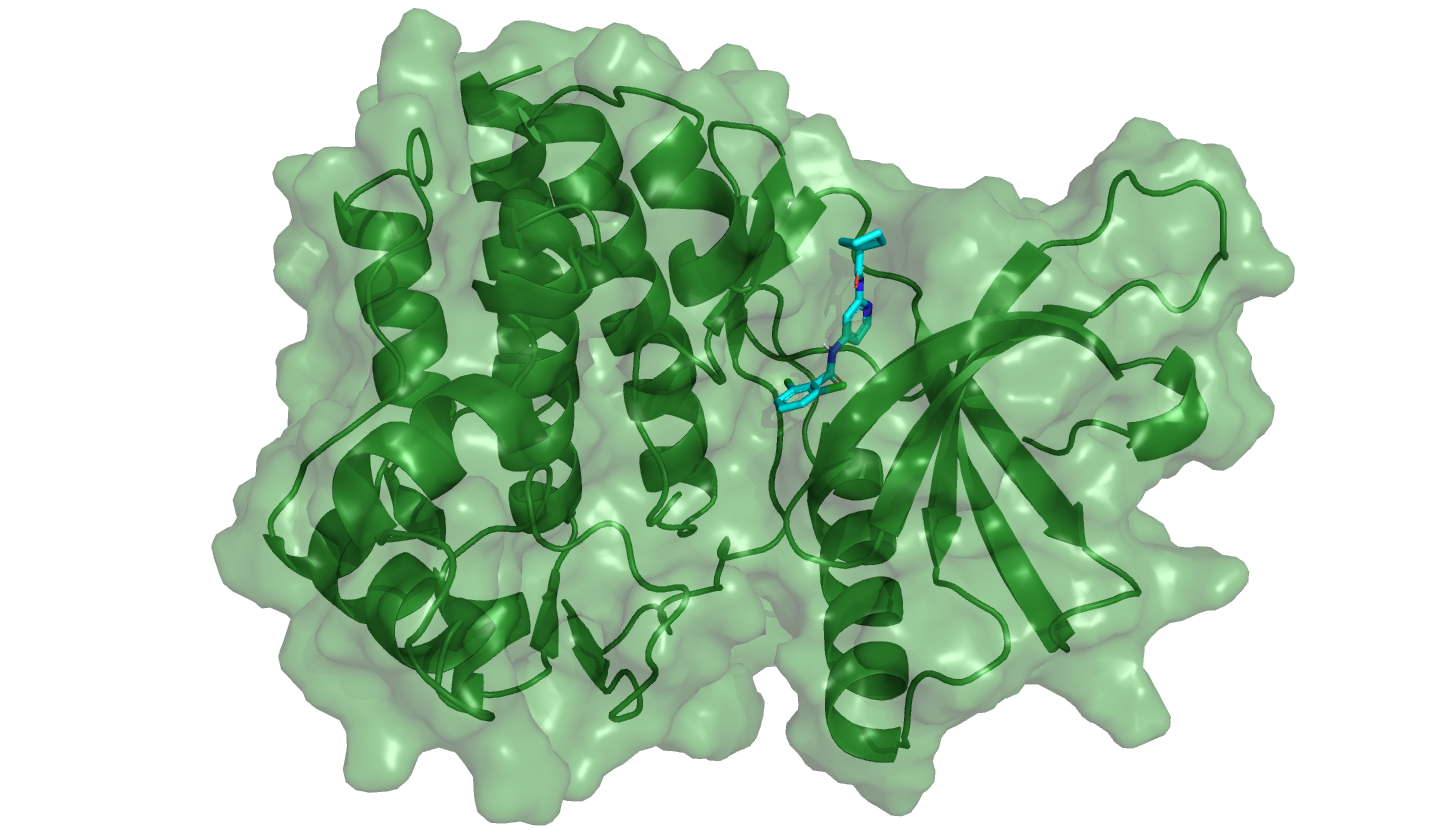
\includegraphics[width=\linewidth]{04_fep/inputs/tut_imgs/tyk2_protlig.png}
\caption{Tyrosine kinase 2 (TYK2) structure with bound ligand
(ejm\_48).}
\label{tyk2_bound_fig}
\end{figure}


Typically in FEP the goal is to predict free energies of binding for a
collection of ligands (normally 10-20). Although methods exist (such as
absolute FEP) that can predict these energies directly (i.e. $\Delta$Gbind),
these are often complicated and computationally expensive. (relative)
FEP uses a basic rule in thermodynamics that dictates that, given a
thermodynamic cycle, the net energy must always be 0. FEP allows users
to compute the $\Delta\Delta$G of binding between two ligands through this mechanism
(see figure \ref{thermodynamic_cycle_fig}).

\begin{figure}[htp]
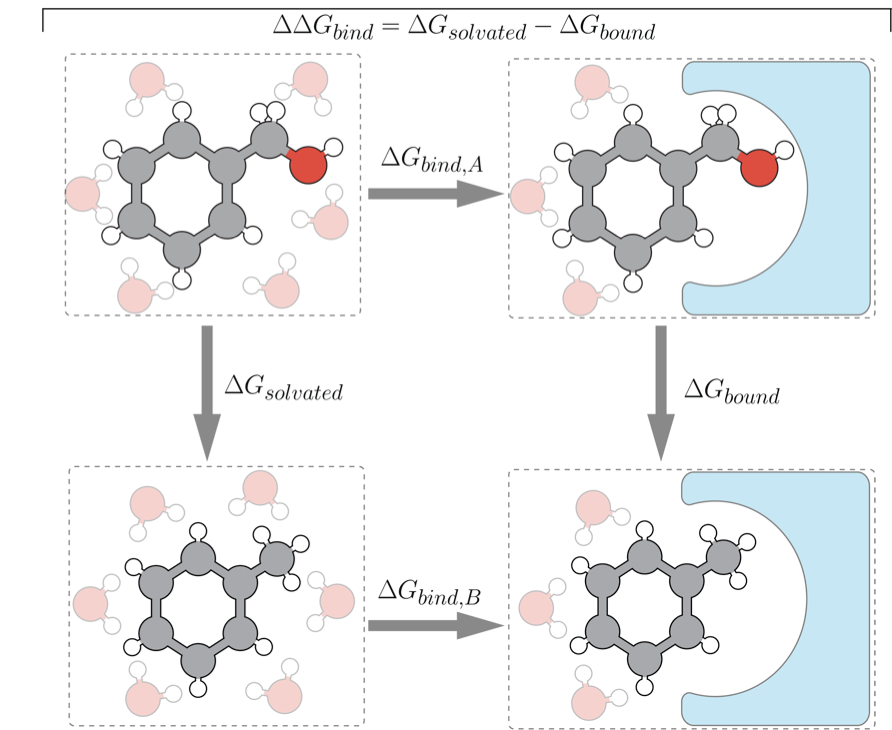
\includegraphics[width=\linewidth]{04_fep/inputs/tut_imgs/therm_cycle.png}
\caption{Thermodynamic cycle that allows FEP practicioners to
compute relative energies of binding. Because the difference between the
vertical legs equals the difference between the horizontal legs, we can
circumvent predicting $\Delta$G$_{bind}$ directly, but instead compute $\Delta\Delta$G$_{bind}$ by
transforming between two ligands in both the solvated and bound phase.}
\label{thermodynamic_cycle_fig}
\end{figure}

Because \emph{relative} energies are calculated, pairs of ligands have to be transformed into one another in both the fee and bound phase (hence the name free energy \emph{perturbation}. Typically, smaller (i.e. fewer heavy atoms) transformations are more reliable which means
that for a ligand series it is recommended to selectively make combinations of
ligands to cover the whole series. In FEP, this is done this using
\emph{perturbation networks}, typically generated by FEP softwares.
Although generating these networks can be done by hand, it is typically
better to do it programmatically to save time and create more optimal networks
(transformation reliability does not depend just on transformation size,
but also on a series of other unfavourable moiety transformations).

\subsubsection{Setting up a FEP calculation using BioSimSpace}

BioSimSpace allows users to set up and run a FEP calculation with just a
few lines of code (and input files). First, BioSimSpace is imported and
and input structures are read:

\begin{python}
import BioSimSpace as BSS
ligand_1 = BSS.IO.readMolecules("ligand_1.mol2")[0]
ligand_2 = BSS.IO.readMolecules("ligand_2.mol2")[0]
protein = BSS.IO.readMolecules("protein.pdb")[0]
\end{python}

\noindent Input molecules are parameterised:

\begin{python}
ligand_1 = BSS.Parameters.gaff2(ligand_1).getMolecule()
ligand_2 = BSS.Parameters.gaff2(ligand_2).getMolecule()
protein = BSS.Parameters.ff14sb(protein).getMolecule()
\end{python}

\noindent Because one ligand is transforming to the other, they need to be
well aligned. This can be done by:

\begin{python}
atom_mapping = BSS.Align.matchAtoms(ligand_1, ligand_2)
ligand_1 = BSS.Align.rmsdAlign(ligand_1, ligand_2, 
                                     atom_mapping)
\end{python}

\noindent Now `merged' molecule (i.e. a molecule that we can
transform in a way such that the endpoints are either input ligands) has to be made. Adding this merged structure into the protein structure can be done simply by addition; the complete system can then be solvated.

\begin{python}
merged = BSS.Align.merge(ligand_1, ligand_2)
system = merged + protein
system_solvated = BSS.Solvent.tip3p(molecule=system, 
                box=3*[10*BSS.Units.Length.nanometer])
\end{python}

\noindent At which point all structures necessary for a FEP run are created. A FEP protocol can be set by:

\begin{python}
protocol = BSS.Protocol.FreeEnergy()
\end{python}

\noindent Note that calling no arguments sets the default FEP protocol. BioSimSpace can set up all necessary files by:

\begin{python}
freenrg = BSS.FreeEnergy.Binding(solvated, protocol, 
                                work_dir="./output")
\end{python}

\noindent Running the FEP calculation is done by:

\begin{python}
freenrg.run() # this call will run the simulation
free_energy = freenrg.analyse()
\end{python}

\noindent Note that this only makes sense on a workstation with GPUs or GPU cloud resources or a GPU cluster. 

\subsubsection{Workflow of a BioSimSpace FEP pipeline}

Because a single FEP simulation typically takes hours to run on a
single GPU (depending on settings and hardware), FEP is usually run on a
computing cluster (or HPC/ cloud service). This allows practitioners to
run many simulations at the same time, turning an FEP pipeline into a
process that takes just several days (or even fewer) instead of weeks (or
even more).

Given a protein input file and a series of ligand input files, we will
be using a Jupyter Notebook that uses LOMAP to generate a perturbation
network for us. This notebook will also write all files necessary to
further prepare our FEP simulations. Because preparing ligands and
proteins for FEP can already require some heavy computation, this will
be the first process that will run on a cluster. Then, after running and
processing the FEP outputs, we can download the results back to our
local workstation. There, the analysis notebook uses FreeEnergyAnalysis
to process FEP predictions and generate plots.

\begin{figure}[htp]
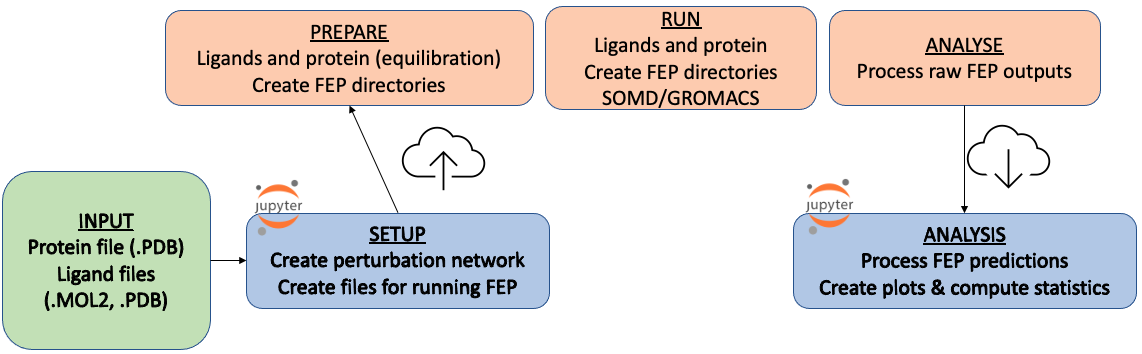
\includegraphics[width=\linewidth]{04_fep/inputs/tut_imgs/fep_pipeline.png}
\caption{Schematic of the FEP pipeline in this tutorial. Whereas blue boxes
represent notebooks run on a local machine, orange boxes represent
python scripts run sequentially on a computing cluster.}
\label{fep_pipeline_fig}
\end{figure}


\subsubsection{Generating a perturbation network to run FEP on a congeneric series of ligands}

For this step, open the jupyter notebook \textbf{setup\_fep.ipynb}. If
you would like to use your own ligands and protein, you can put these in
\texttt{inputs/ligands/} and \texttt{inputs/protein/}, respectively.

After running all the cells in this notebook, the folder
\texttt{./execution\_model/} will contain everything needed to run FEP
in parallel on your cluster. To move this folder to your cluster, you
can use for instance SCP:

\begin{lstlisting}
$ scp -r execution_model uname@cluster.address:/path/to/folder
\end{lstlisting}

\noindent \emph{Note: if a computing cluster shares its file system with the local workstation the above step is not necessarily needed.}


\subsubsection{Running FEP on a computing cluster using
BioSimSpace}

The folder \texttt{./execution\_model/} contains several scripts and
folders, of which the most important are:

\begin{itemize}
\item
  \texttt{processFEP-slurm.sh} and \texttt{processFEP-lsf.sh}: running
  either of these scripts will submit all simulation jobs (depending on the
  cluster setup). Note that there are several parameters at the top of
  these scripts that have to be set (by e.g. a system administrator)
  that will inform BioSimSpace of all relevant paths to software
  dependencies and other important matters.
\item
  \texttt{./scripts/} contains all necessary scripts to run FEP with
  BioSimSpace. Advanced users can tweak more settings in these.
\end{itemize}

If everything has been set up correctly, running:

\begin{lstlisting}
$ bash processFEP-slurm.sh
\end{lstlisting}

will start the whole FEP job submission (for SLURM clusters). First, all systems will be
prepared, then run and then analysed (see figure \ref{fep_pipeline_fig}). When jobs finish, FEP predictions will be written to \texttt{./outputs/SOMD/summary.csv} (in case of SOMD
engine). Logfiles for seeing process outputs can be found in
\texttt{./logs/}. Additionally, perturbations that were simulated
successfully will have an \emph{overlap matrix} figure saved to
\texttt{./logs/} (in case of SOMD); these can be checked to check if perturbations were likely to be reliable per simulation leg. \cite{mey2020best}

For the final analysis, only \texttt{./outputs/SOMD/summary.csv} is required. Thus, this file has to be downloaded back to the local workstation; using SCP again (from the workstation, i.e. not logged into the cluster):

\begin{lstlisting}
$ scp uname@cluster.address:/path/to/folder\ /outputs/SOMD/summary.csv .
\end{lstlisting}


\subsubsection{Analysing FEP results}

For this step, open the jupyter notebook \textbf{analyse\_fep.ipynb}.
Running cells in this notebook will generate typical FEP figures
(barplots and scatterplots); if you have missing or failed
perturbations, the script should be able to work out an optimal
prediction (although at some point with enough missing FEP predictions,
ligands will of course be missing). If you happen to have experimental
affinity values, you can validate how accurate your FEP predictions are.

An example result from this notebook is a barplot:

\begin{figure}[htp]
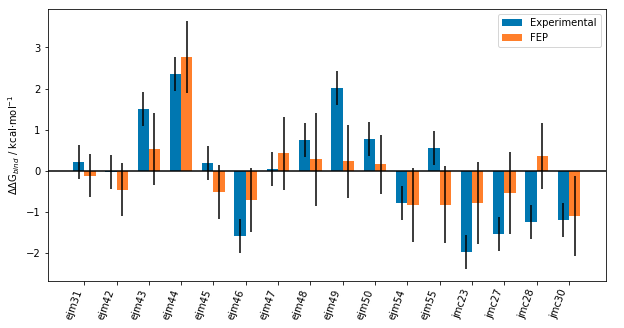
\includegraphics[width=\linewidth]{04_fep/inputs/tut_imgs/fep_barplot.png}
\caption{Example barplot depicting FEP results, generated with the analysis jupyter notebook included in this tutorial.}
\label{fep_barplot_fig}
\end{figure}



% %%%% YOU CAN USE THIS BLOCK FOR PYTHON:
% \begin{python}
% import numpy as np
    
% def incmatrix(genl1,genl2):
%     M = []
%     m = len(genl1)  # comment 
%     for i in m:
%         M.append(i)
    
%     return M
% \end{python}

% %%%% YOU CAN USE THIS BLOCK FOR BASH:
% \begin{lstlisting}
% $ command -arg1 -arg2 -arg3 -arg4 -arg5 -arg6 > output.file 2> err.file
% \end{lstlisting}

% %%%% YOU CAN USE THE SAME BLOCK FOR TEXT (e.g. STDOUT):
% \begin{lstlisting}[columns=flexible]
% this is an example of a message printed to StdOut!
% \end{lstlisting}

% %%%% FOR LARGE CHUNKS OF TEXTS, USE \scriptsize{} (OR EVEN \tiny{}) TO MAKE IT FIT THE COLUMNS
% {\scriptsize
% \begin{lstlisting}[columns=flexible]

% %VERSION  VERSION_STAMP = V0001.000  DATE = 06/30/15  11:44:23                  
% %FLAG TITLE                                                                     
% %FORMAT(20a4)                                                                   
% ACE                                                                             
% %FLAG POINTERS                                                                  
% %FORMAT(10I8)                                                                   
%     1912       9    1902       9      25      11      43      24       0       0
%     2619     633       9      11      24      13      21      20      10       1
%       0       0       0       0       0       0       0       1      10       0
%       0
% %FLAG ATOM_NAME                                                                 
% %FORMAT(20a4)                                                                   
% HH31CH3 HH32HH33C   O   N   H   CA  HA  CB  HB1 HB2 HB3 C   O   N   H   CH3 HH31
% HH32HH33O   H1  H2  O   H1  H2  O   H1  H2  O   H1  H2  O   H1  H2  O   H1  H2  
% O   H1  H2  O   H1  H2  O   H1  H2  O   H1  H2  O   H1  H2  O   H1  H2  O   H1  
% H2  O   H1  H2  O   H1  H2  O   H1  H2  O   H1  H2  O   H1  H2  O   H1  H2  O   
% H1  H2  O   H1  H2  O   H1  H2  O   H1  H2  O   H1  H2  O   H1  H2  O   H1  H2  
% O   H1  H2  O   H1  H2  O   H1  H2  O   H1  H2  O   H1  H2  O   H1  H2  O   H1  
% H2  O   H1  H2  O   H1  H2  O   H1  H2  O   H1  H2  O   H1  H2  O   H1  H2  O   
% H1  H2  O   H1  H2  O   H1  H2  O   H1  H2  O   H1  H2  O   H1  H2  O   H1  H2 
% \end{lstlisting}
% }


\section{Checklists}
Tutorials do not necessarily require the use of a checklist as in Best Practices documents; however, they can include these if desired.
Several useful checklist formats are available, with examples presented in \texttt{sample-document.tex} in \url{github.com/livecomsjournal/article_templates/templates}.
One example is shown here.

% Here is a single-column checklist that consists of multiple sub-checklists
\begin{Checklists}

\begin{checklist}{A list}
\textbf{Single-column checklists are also straightforward by removing the asterisk}
\begin{itemize}
\item First thing let's do an item which breaks across lines to see how that looks
\item Also remember
\item And finally
\end{itemize}
\end{checklist}

\begin{checklist}{Another list}
\textbf{This is some further description.}
\begin{itemize}
\item First thing
\item Also remember
\item And finally
\end{itemize}
\end{checklist}

\end{Checklists}








\section{Author Contributions}
%%%%%%%%%%%%%%%%
% This section mustt describe the actual contributions of
% author. Since this is an electronic-only journal, there is
% no length limit when you describe the authors' contributions,
% so we recommend describing what they actually did rather than
% simply categorizing them in a small number of
% predefined roles as might be done in other journals.
%
% See the policies ``Policies on Authorship'' section of https://livecoms.github.io
% for more information on deciding on authorship and author order.
%%%%%%%%%%%%%%%%

(Explain the contributions of the different authors here)

% We suggest you preserve this comment:
For a more detailed description of author contributions,
see the GitHub issue tracking and changelog at \githubrepository.

\section{Other Contributions}
%%%%%%%%%%%%%%%
% You should include all people who have filed issues that were
% accepted into the paper, or that upon discussion altered what was in the paper.
% Multiple significant contributions might mean that the contributor
% should be moved to authorship at the discretion of the a
%
% See the policies ``Policies on Authorship'' section of https://livecoms.github.io for
% more information on deciding on authorship and author order.
%%%%%%%%%%%%%%%

(Explain the contributions of any non-author contributors here)
% We suggest you preserve this comment:
For a more detailed description of contributions from the community and others, see the GitHub issue tracking and changelog at \githubrepository.

\section{Potentially Conflicting Interests}
%%%%%%%
%Declare any potentially competing interests, financial or otherwise
%%%%%%%

Declare any potentially conflicting interests here, whether or not they pose an actual conflict in your view.

\section{Funding Information}
%%%%%%%
% Authors should acknowledge funding sources here. Reference specific grants.
%%%%%%%
FMS acknowledges the support of NSF grant CHE-1111111.

\section*{Author Information}
\makeorcid

\bibliography{references}

%%%%%%%%%%%%%%%%%%%%%%%%%%%%%%%%%%%%%%%%%%%%%%%%%%%%%%%%%%%%
%%% APPENDICES
%%%%%%%%%%%%%%%%%%%%%%%%%%%%%%%%%%%%%%%%%%%%%%%%%%%%%%%%%%%%

%\appendix


\end{document}